% Visual Diagrams for Part I: Foundations
% To be included in appropriate chapters

% ============================================================================
% Chapter 1: The Approximation Advantage
% ============================================================================

% Figure 1.1: Space-Accuracy Tradeoff
\begin{figure}[h]
\centering
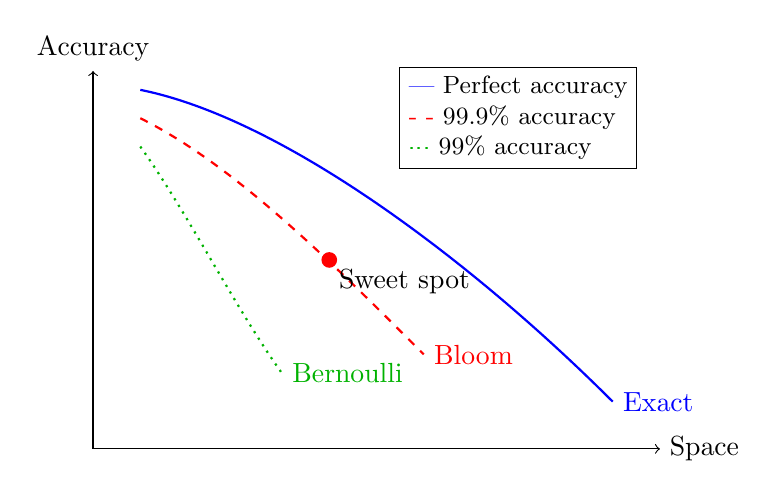
\begin{tikzpicture}[scale=1.2]
    % Axes
    \draw[->] (0,0) -- (6,0) node[right] {Space};
    \draw[->] (0,0) -- (0,4) node[above] {Accuracy};
    
    % Curves
    \draw[thick, blue] (0.5,3.8) .. controls (2,3.5) and (4,2) .. (5.5,0.5) 
        node[right] {Exact};
    \draw[thick, red, dashed] (0.5,3.5) .. controls (1.5,3) and (2.5,2) .. (3.5,1)
        node[right] {Bloom};
    \draw[thick, green!70!black, dotted] (0.5,3.2) .. controls (1,2.5) and (1.5,1.5) .. (2,0.8)
        node[right] {Bernoulli};
    
    % Points of interest
    \node[circle, fill=red, inner sep=2pt] at (2.5,2) {};
    \node[below right] at (2.5,2) {Sweet spot};
    
    % Legend box
    \node[draw, align=left, font=\small] at (4.5,3.5) {
        \textcolor{blue}{—} Perfect accuracy\\
        \textcolor{red}{- -} 99.9\% accuracy\\
        \textcolor{green!70!black}{···} 99\% accuracy
    };
\end{tikzpicture}
\caption{The space-accuracy tradeoff: Bernoulli types achieve massive space savings with minimal accuracy loss}
\label{fig:space-accuracy}
\end{figure}

% Figure 1.2: Bloom Filter Operation
\begin{figure}[h]
\centering
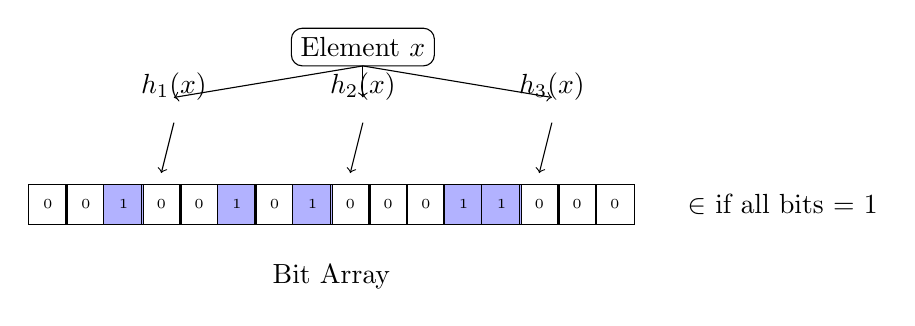
\begin{tikzpicture}[scale=0.8]
    % Bit array
    \foreach \i in {0,...,15} {
        \pgfmathparse{int(mod(\i+3,5)==0 || mod(\i+7,6)==0)}
        \ifnum\pgfmathresult=1
            \node[rectangle, draw, fill=blue!30, minimum size=0.5cm] at (\i*0.6,0) {\tiny 1};
        \else
            \node[rectangle, draw, minimum size=0.5cm] at (\i*0.6,0) {\tiny 0};
        \fi
    }
    
    % Hash functions
    \node[above] at (2,1.5) {$h_1(x)$};
    \draw[->] (2,1.3) -- (1.8,0.5);
    
    \node[above] at (5,1.5) {$h_2(x)$};
    \draw[->] (5,1.3) -- (4.8,0.5);
    
    \node[above] at (8,1.5) {$h_3(x)$};
    \draw[->] (8,1.3) -- (7.8,0.5);
    
    % Input
    \node[draw, rounded corners] at (5,2.5) {Element $x$};
    \draw[->] (5,2.2) -- (2,1.7);
    \draw[->] (5,2.2) -- (5,1.7);
    \draw[->] (5,2.2) -- (8,1.7);
    
    % Labels
    \node[below] at (4.5,-0.8) {Bit Array};
    \node[right] at (10,0) {$\in$ if all bits = 1};
\end{tikzpicture}
\caption{Bloom filter: Multiple hash functions map elements to bit positions}
\label{fig:bloom-operation}
\end{figure}

% ============================================================================
% Chapter 2: From Hashing to Hiding
% ============================================================================

% Figure 2.1: Hash Function Properties
\begin{figure}[h]
\centering
\begin{tikzpicture}[scale=1]
    % Input space
    \draw[ellipse, minimum width=3cm, minimum height=4cm, draw] at (0,0) {};
    \node[above] at (0,2.2) {Input Space};
    
    % Output space
    \draw[ellipse, minimum width=3cm, minimum height=3cm, draw, fill=gray!20] at (6,0) {};
    \node[above] at (6,1.7) {Hash Space};
    
    % Mappings
    \foreach \y in {1.5,0.5,-0.5,-1.5} {
        \node[circle, fill=blue, inner sep=1pt] (a\y) at (-0.5,\y) {};
    }
    \foreach \y in {1,0,-1} {
        \node[circle, fill=red, inner sep=1pt] (b\y) at (5.5,\y) {};
    }
    
    % Arrows showing many-to-one
    \draw[->] (a1.5) to[out=20,in=160] (b1);
    \draw[->] (a0.5) to[out=10,in=170] (b1);
    \draw[->] (a-0.5) to[out=0,in=180] (b0);
    \draw[->] (a-1.5) to[out=-10,in=-170] (b-1);
    
    % Properties
    \node[draw, align=left, below] at (3,-3) {
        \textbf{Properties:}\\
        • Deterministic\\
        • Uniform distribution\\
        • Avalanche effect\\
        • One-way
    };
\end{tikzpicture}
\caption{Cryptographic hash functions provide uniform, irreversible mappings}
\label{fig:hash-properties}
\end{figure}

% Figure 2.2: From Deterministic to Probabilistic
\begin{figure}[h]
\centering
\begin{tikzpicture}[scale=1.2]
    % Traditional (deterministic)
    \node[draw, rectangle] (input1) at (0,2) {Query: "covid"};
    \node[draw, rectangle, fill=blue!20] (hash1) at (3,2) {$h($"covid"$)$};
    \node[draw, rectangle] (output1) at (6,2) {0x3f2a...};
    \draw[->] (input1) -- (hash1);
    \draw[->] (hash1) -- (output1);
    \node[above] at (3,2.5) {Deterministic};
    
    % Bernoulli (probabilistic)
    \node[draw, rectangle] (input2) at (0,0) {Query: "covid"};
    \node[draw, rectangle, fill=green!20] (hash2) at (3,0) {$\tilde{h}($"covid"$)$};
    \node[draw, cloud, cloud puffs=10, minimum width=2cm, minimum height=1cm] (output2) at (6,0) {Random noise};
    \draw[->] (input2) -- (hash2);
    \draw[->] (hash2) -- (output2);
    \node[below] at (3,-0.5) {Probabilistic};
    
    % Comparison
    \draw[dashed, red] (6.5,1.5) -- (6.5,0.5);
    \node[right, red] at (6.7,1) {Different!};
\end{tikzpicture}
\caption{Bernoulli encoding: Same input produces different outputs each time}
\label{fig:deterministic-vs-probabilistic}
\end{figure}

% ============================================================================
% Chapter 3: The Privacy Problem
% ============================================================================

% Figure 3.1: Information Leakage Channels
\begin{figure}[h]
\centering
\begin{tikzpicture}[scale=1]
    % User
    \node[draw, circle, minimum size=1cm] (user) at (0,0) {User};
    
    % Server
    \node[draw, rectangle, minimum width=2cm, minimum height=3cm, fill=gray!20] (server) at (8,0) {Server};
    
    % Query flow
    \draw[->, thick] (user) -- node[above] {Query} (server);
    
    % Leakage channels
    \draw[->, red, dashed] (3,0.5) -- (3,2) node[above] {Frequency};
    \draw[->, red, dashed] (4,0.5) -- (4,2) node[above] {Timing};
    \draw[->, red, dashed] (5,0.5) -- (5,2) node[above] {Correlation};
    \draw[->, red, dashed] (6,0.5) -- (6,2) node[above] {Volume};
    \
    % Adversary
    \node[draw, ellipse, fill=red!20] (adversary) at (5,3) {Adversary};
    \draw[->, red] (3,2) -- (adversary);
    \draw[->, red] (4,2) -- (adversary);
    \draw[->, red] (5,2) -- (adversary);
    \draw[->, red] (6,2) -- (adversary);
    
    % What adversary learns
    \node[draw, align=left, below] at (5,-2) {
        \textbf{Adversary learns:}\\
        • User interests\\
        • Search patterns\\
        • Investigation targets\\
        • Activity timeline
    };
\end{tikzpicture}
\caption{Multiple channels leak information even with encrypted queries}
\label{fig:leakage-channels}
\end{figure}

% Figure 3.2: Privacy-Functionality-Efficiency Triangle
\begin{figure}[h]
\centering
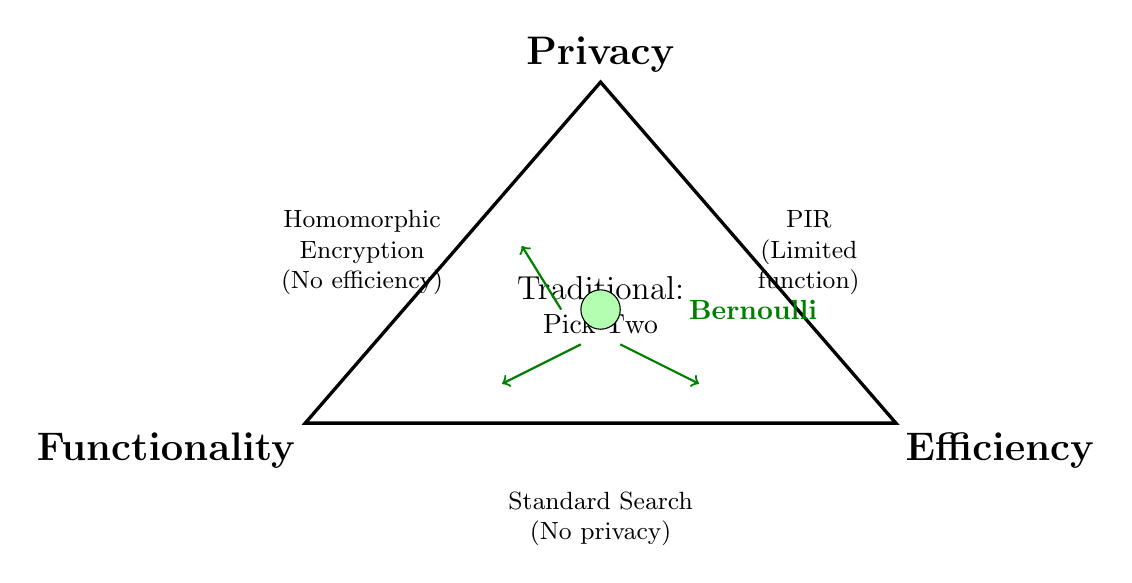
\begin{tikzpicture}[scale=2.5]
    % Triangle vertices
    \coordinate (P) at (0,1.732);
    \coordinate (F) at (-1.5,0);
    \coordinate (E) at (1.5,0);
    
    % Draw triangle
    \draw[very thick] (P) -- (F) -- (E) -- cycle;
    
    % Vertex labels
    \node[above] at (P) {\Large \textbf{Privacy}};
    \node[below left] at (F) {\Large \textbf{Functionality}};
    \node[below right] at (E) {\Large \textbf{Efficiency}};
    
    % Center
    \node[align=center] at (0,0.6) {\large Traditional:\\Pick Two};
    
    % Edge descriptions
    \node[left, align=center, font=\small] at (-0.75,0.866) {Homomorphic\\Encryption\\(No efficiency)};
    \node[right, align=center, font=\small] at (0.75,0.866) {PIR\\(Limited\\function)};
    \node[below, align=center, font=\small] at (0,-0.3) {Standard Search\\(No privacy)};
    
    % Our solution (center)
    \node[draw, circle, fill=green!30, minimum size=0.5cm] at (0,0.577) {};
    \node[right, green!50!black] at (0.4,0.577) {\textbf{Bernoulli}};
    
    % Arrows showing balance
    \draw[->, green!50!black, thick] (-0.2,0.577) -- (-0.4,0.9);
    \draw[->, green!50!black, thick] (-0.1,0.4) -- (-0.5,0.2);
    \draw[->, green!50!black, thick] (0.1,0.4) -- (0.5,0.2);
\end{tikzpicture}
\caption{The fundamental tradeoff: Bernoulli types achieve balance through approximation}
\label{fig:privacy-triangle}
\end{figure}

% ============================================================================
% Chapter 4: Building Your First Oblivious System
% ============================================================================

% Figure 4.1: System Architecture
\begin{figure}[h]
\centering
\begin{tikzpicture}[scale=1,
    box/.style={draw, rectangle, minimum width=2cm, minimum height=1cm},
    data/.style={draw, cylinder, shape border rotate=90, minimum width=1.5cm, minimum height=1cm}]
    
    % Client side
    \node[box] (client) at (0,3) {Client App};
    \node[box, fill=blue!20] (encoder) at (0,1.5) {Encoder};
    \node[box, fill=blue!20] (decoder) at (0,0) {Decoder};
    
    % Network
    \node[cloud, draw, cloud puffs=12, minimum width=3cm, minimum height=2cm] (network) at (4,1.5) {Network};
    
    % Server side
    \node[box, fill=red!20] (oblivious) at (8,3) {Oblivious Index};
    \node[data] (storage) at (8,1.5) {Bloom Filters};
    \node[box] (processor) at (8,0) {Query Processor};
    
    % Connections
    \draw[->] (client) -- (encoder);
    \draw[->] (encoder) -- (network);
    \draw[->] (network) -- (oblivious);
    \draw[<->] (oblivious) -- (storage);
    \draw[->] (oblivious) -- (processor);
    \draw[->] (processor) -- (network);
    \draw[->] (network) -- (decoder);
    \draw[->] (decoder) -- (client);
    
    % Adversary observation
    \node[draw, ellipse, fill=gray!30] (adversary) at (4,4) {Adversary};
    \draw[dashed, ->] (network) -- (adversary);
    \node[right] at (5,4) {Sees only noise!};
    
    % Labels
    \node[align=center, below] at (0,-1) {\textbf{Client}\\(Trusted)};
    \node[align=center, below] at (8,-1) {\textbf{Server}\\(Untrusted)};
\end{tikzpicture}
\caption{Oblivious system architecture: Privacy through encoded queries}
\label{fig:system-architecture}
\end{figure}

% Figure 4.2: Query Processing Flow
\begin{figure}[h]
\centering
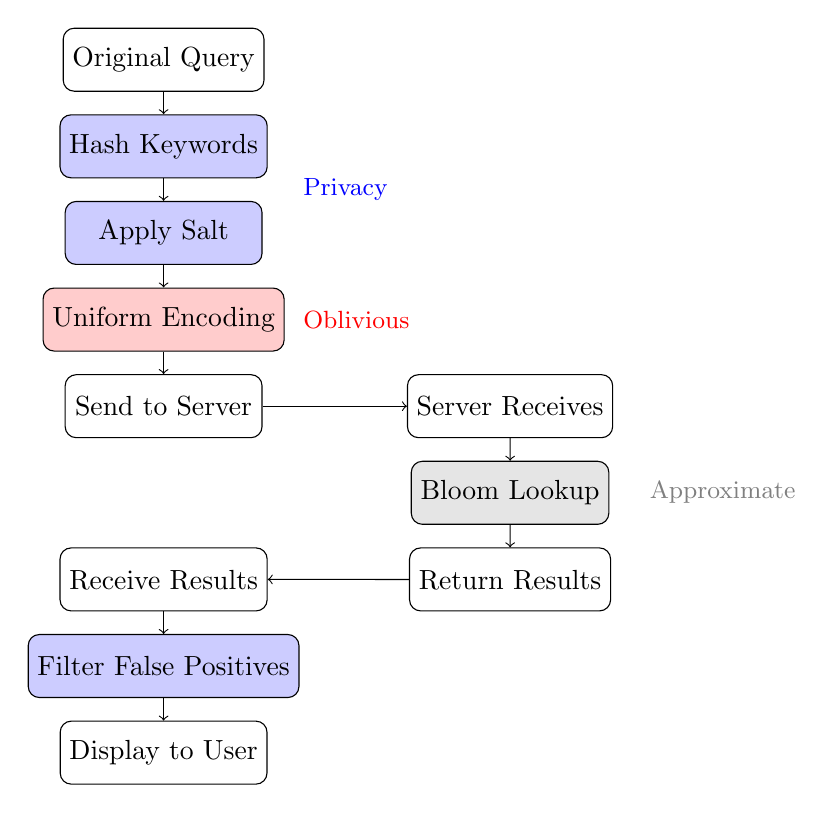
\begin{tikzpicture}[scale=1.1,
    process/.style={draw, rectangle, rounded corners, minimum width=2.5cm, minimum height=0.8cm}]
    
    % Query flow
    \node[process] (q1) at (0,4) {Original Query};
    \node[process, fill=blue!20] (q2) at (0,3) {Hash Keywords};
    \node[process, fill=blue!20] (q3) at (0,2) {Apply Salt};
    \node[process, fill=red!20] (q4) at (0,1) {Uniform Encoding};
    \node[process] (q5) at (0,0) {Send to Server};
    
    % Arrows
    \draw[->] (q1) -- (q2);
    \draw[->] (q2) -- (q3);
    \draw[->] (q3) -- (q4);
    \draw[->] (q4) -- (q5);
    
    % Server processing
    \node[process] (s1) at (4,0) {Server Receives};
    \node[process, fill=gray!20] (s2) at (4,-1) {Bloom Lookup};
    \node[process] (s3) at (4,-2) {Return Results};
    
    % Arrows
    \draw[->] (q5) -- (s1);
    \draw[->] (s1) -- (s2);
    \draw[->] (s2) -- (s3);
    
    % Client decoding
    \node[process] (d1) at (0,-2) {Receive Results};
    \node[process, fill=blue!20] (d2) at (0,-3) {Filter False Positives};
    \node[process] (d3) at (0,-4) {Display to User};
    
    % Arrows
    \draw[->] (s3) -- (d1);
    \draw[->] (d1) -- (d2);
    \draw[->] (d2) -- (d3);
    
    % Annotations
    \node[right, font=\small, text=blue] at (1.5,2.5) {Privacy};
    \node[right, font=\small, text=red] at (1.5,1) {Oblivious};
    \node[right, font=\small, text=gray] at (5.5,-1) {Approximate};
\end{tikzpicture}
\caption{Query processing: Each step adds privacy while maintaining functionality}
\label{fig:query-flow}
\end{figure}

% Figure 4.3: Performance Comparison
\begin{figure}[h]
\centering
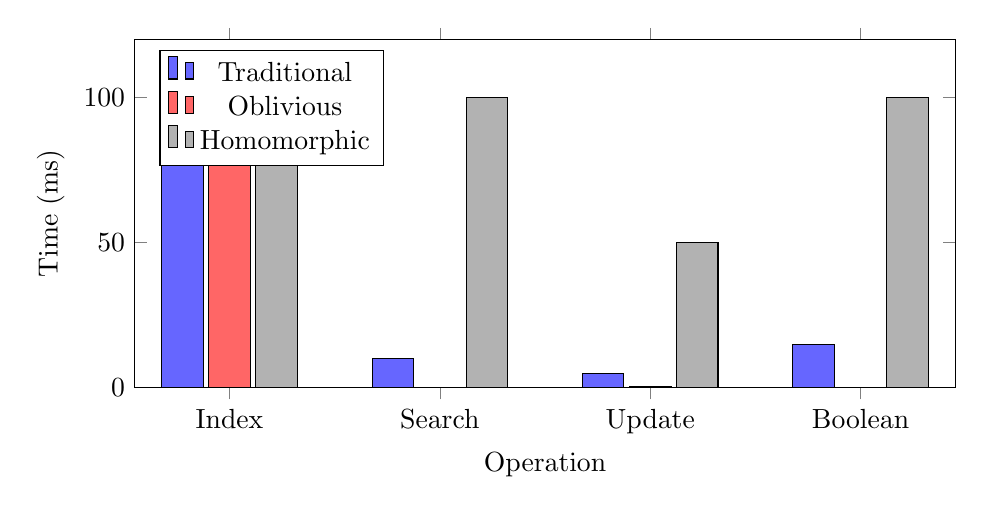
\begin{tikzpicture}[scale=1]
    \begin{axis}[
        ybar,
        width=12cm,
        height=6cm,
        ylabel={Time (ms)},
        xlabel={Operation},
        symbolic x coords={Index,Search,Update,Boolean},
        xtick=data,
        legend pos=north west,
        ymin=0,
        ymax=120,
        bar width=15pt,
        enlarge x limits=0.15,
    ]
    
    % Traditional
    \addplot[fill=blue!60] coordinates {
        (Index,100) (Search,10) (Update,5) (Boolean,15)
    };
    
    % Oblivious
    \addplot[fill=red!60] coordinates {
        (Index,80) (Search,0.05) (Update,0.5) (Boolean,0.1)
    };
    
    % Homomorphic
    \addplot[fill=gray!60] coordinates {
        (Index,100) (Search,100) (Update,50) (Boolean,100)
    };
    
    \legend{Traditional, Oblivious, Homomorphic}
    \end{axis}
\end{tikzpicture}
\caption{Performance comparison: Oblivious achieves sub-millisecond operations}
\label{fig:performance}
\end{figure}

% ============================================================================
% Unified Concepts Diagram
% ============================================================================

\begin{figure}[h]
\centering
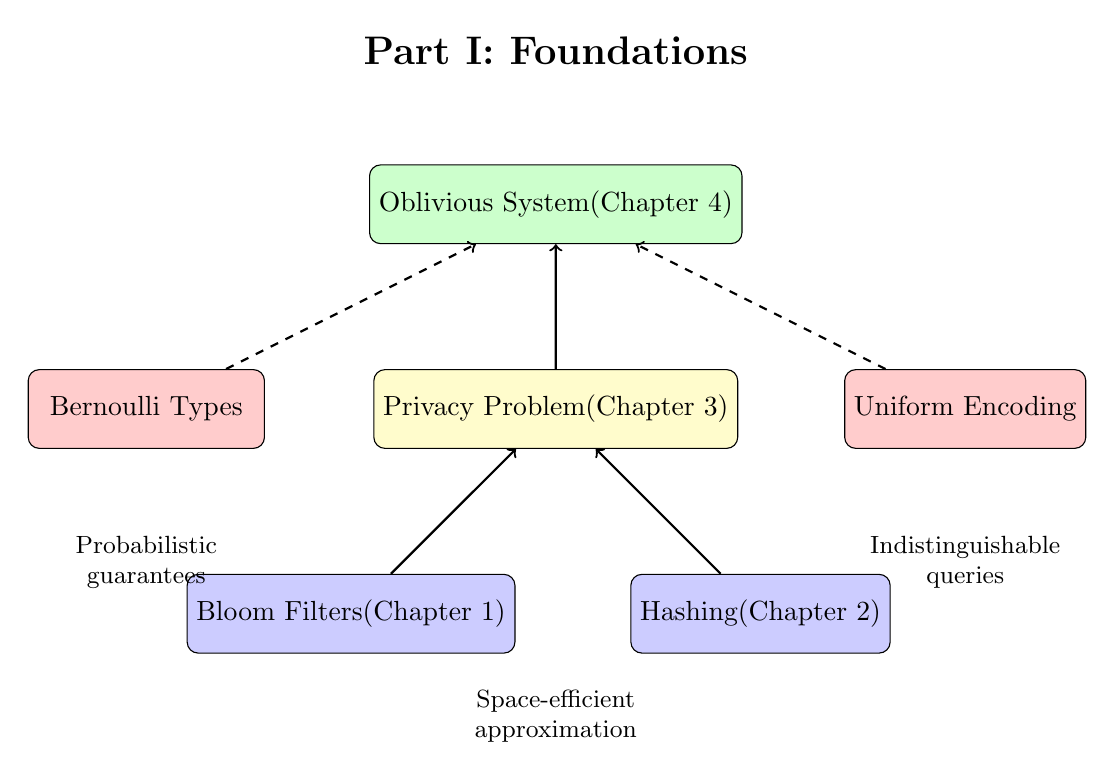
\begin{tikzpicture}[scale=1.3,
    concept/.style={draw, rectangle, rounded corners, minimum width=3cm, minimum height=1cm},
    arrow/.style={->, thick}]
    
    % Layer 1: Foundation
    \node[concept, fill=blue!20] (bloom) at (0,0) {Bloom Filters\\(Chapter 1)};
    \node[concept, fill=blue!20] (hash) at (4,0) {Hashing\\(Chapter 2)};
    
    % Layer 2: Problem
    \node[concept, fill=yellow!20] (privacy) at (2,2) {Privacy Problem\\(Chapter 3)};
    
    % Layer 3: Solution
    \node[concept, fill=green!20] (oblivious) at (2,4) {Oblivious System\\(Chapter 4)};
    
    % Connections
    \draw[arrow] (bloom) -- (privacy);
    \draw[arrow] (hash) -- (privacy);
    \draw[arrow] (privacy) -- (oblivious);
    
    % Side concepts
    \node[concept, fill=red!20] (bernoulli) at (-2,2) {Bernoulli Types};
    \node[concept, fill=red!20] (encoding) at (6,2) {Uniform Encoding};
    
    \draw[arrow, dashed] (bernoulli) -- (oblivious);
    \draw[arrow, dashed] (encoding) -- (oblivious);
    
    % Annotations
    \node[align=center, font=\small] at (2,-1) {Space-efficient\\approximation};
    \node[align=center, font=\small] at (-2,0.5) {Probabilistic\\guarantees};
    \node[align=center, font=\small] at (6,0.5) {Indistinguishable\\queries};
    
    % Title
    \node[font=\Large\bfseries] at (2,5.5) {Part I: Foundations};
\end{tikzpicture}
\caption{Conceptual flow through Part I: From approximation to oblivious computing}
\label{fig:part1-overview}
\end{figure}